\documentclass{llncs}
\usepackage{times}
\usepackage{graphicx}
\usepackage{multirow}
\usepackage{colortbl}
\usepackage{rotating}
\usepackage{array}
\usepackage[usenames,dvipsnames]{xcolor}
%\usepackage{flushend}

\usepackage{ifthen}
\usepackage{amssymb}
\newboolean{showcomments}
\setboolean{showcomments}{true} % toggle to show or hide comments

\ifthenelse{\boolean{showcomments}}
  {\newcommand{\nb}[2]{
    \fcolorbox{gray}{yellow}{\bfseries\sffamily\scriptsize#1}
    {\sf\small$\blacktriangleright$\textit{#2}$\blacktriangleleft$}
   }
   \newcommand{\version}{\emph{\scriptsize$-$working$-$}}
  }
  {\newcommand{\nb}[2]{}
   \newcommand{\version}{}
  }

\ifthenelse{\boolean{showcomments}}
  {\newcommand{\rev}[1]{\textcolor{red}{#1}}}
  {\newcommand{\rev}[1]{#1}}

\newcommand\jordi[1]{\nb{Jordi}{#1}}
\newcommand\javier[1]{\nb{Javier}{#1}}

\hyphenation{op-tical net-works semi-conduc-tor}

%\usepackage[nospace]{cite}

\setlength{\textfloatsep}{2mm}
%\setlength{\intextsep}{3mm}
%\setlength{\belowcaptionskip}{-0mm}

%\clubpenalty = 10000
%\widowpenalty = 10000
%\displaywidowpenalty = 10000

\begin{document}
\title{Specification and Application of Governance Rules in Software Development\thanks{This work has been supported by the European Commission under the ICT Policy Support Programme, grant no. 317859.}}
\author{Javier Luis C\'anovas Izquierdo, Jordi Cabot}

\institute{AtlanMod, \'Ecole des Mines de Nantes -- INRIA -- LINA, Nantes, France\\ \email{\{javier.canovas,jordi.cabot\}@inria.fr}}

\maketitle

%\vspace{-0.5cm}

\begin{abstract}
Any software development project is decomposed into a series of tasks that must be properly prioritized and managed for the success of the project. Unfortunately, the rules governing the development process (e.g., describing who can implement a task or deciding which tasks should be completed first) are usually implicit or appear scattered in the project documentation or tools (e.g., tracking-systems, forums, etc.). In this paper we propose to enable the explicit definition of governance rules for development tasks along with complementary support for their application. Making explicit governance rules will provide several important benefits, including improvements in the transparency and sustainability of the project. Furthermore, the support for the rule application will promote traceability (why a decision was made) and the automation of the governance process (i.e., liberating developers from applying the rules manually and avoiding potential inconsistencies). We created a domain-specific language to easily define governance rules, which is illustrated with real open source projects, whereas their application is supported by a tool implemented on top of Mylyn, a project management plug-in for Eclipse, which supports most tracking-systems, thus allowing the use of our approach in most development projects.
\keywords{Decision making, Governance, Collaborative Software Development}
\end{abstract}

%\vspace{-1cm}

\section{Introduction}
\label{sec:introduction}
The development of large-scale software has to cope with a huge number of tasks consisting of either implementing new issues or fixing bugs~\cite{Aranda2009}. Thus, effective and precise prioritization of these tasks is key for the success of the project. For this purpose, each project defines and applies its own set of governance rules, which also define how to contribute in the project and how decisions are made (e.g., which issues have to be implemented or when the next milestone will be). Thus, a governance model enables the coordination of developers in order to advance the project. According to Conway's Law~\cite{Conway1968}, this coordination has a direct impact on the product being built \cite{Herbsleb1999}.  

Governance models makes particularly sense in the context of Open Source System (OSS) development projects \cite{osswatch}, where external developers can participate actively and need to know how they can contribute. However, these projects usually have a methodology very loosely defined (if any)~\cite{McConnell1999} and it is hard to find an explicit system-level design, a project plan, schedule or list of deliverables~\cite{Mockus}. Thus, despite their importance, in practice governance models are hardly ever explicitly defined. This hampers the integration of new developers\footnote{E.g., searching for \emph{how to contribute} in \emph{Stackoverflow} returns more than four thousand results (i.e., $\sim$8\% of the total number of questions)} in the team who must spend some time understanding the ``culture'' of the project \cite{Shibuya2009}. 

%For this purpose, each project defines and applies its own set of governance rules. These rules can be as simple as \emph{team leaders decide the tasks to do} or more complex as \emph{the task to be done will be the one most voted by the developers participating in the project}. Governance rules enable the coordination of developers in order to advance the project. According to Conway's Law~\cite{Conway1968}, this coordination has a direct impact on the product being built \cite{Herbsleb1999}.  

%Despite their importance, in practice governance rules are hardly ever explicitly defined, specially in the context of Open Source Systems (OSS), where the development methodology is very loosely defined (if any)~\cite{McConnell1999} and it is hard to find an explicit system-level design, a project plan, schedule or list of deliverables~\cite{Mockus}. Moreover, the support for enforcing such governance rules is even more limited. This hampers the integration of new developers in the team who must spend some time understanding the ``culture'' of the project \cite{Shibuya2009}. 

The governance model being missing, mechanisms to facilitate the communication and the assignment of work are considered crucial for the success of the development~\cite{Mockus2000,Crowston2012}. Tracking systems (i.e., bug-traking such as Bugzilla\footnote{http://www.bugzilla.org/} and issue-tracking systems such as Mantis\footnote{http://www.mantisbt.org/}) are broadly used to manage the tasks to be performed. Other collaborative tools such as mailing-lists or forums are also used to coordinate the developers involved in the project. While these tools provide a convenient compartmentalization of work and effective means of communication, they fall short in providing adequate support for specifying and applying a governance model (e.g., supporting the voting of tasks, easy tracking of decisions made in the project, etc.). 

Therefore, the explicit definition of a governance model would have several benefits, including improvements in the transparency and sustainability \cite{osswatch}. Moreover, we believe the support for not only the definition but also the application of the governance model would also promote traceability (being able to track why a decision was made and who decided it) and the automation of the governance process (e.g., liberating developers from having to be aware and follow the rules manually, minimizing the risk of inconsitent behaviour in the evolution of the project). 

%Therefore, we believe the explicit definition of a governance model along with the corresponding infrastructure to help developers realize it would have several benefits, including improvements in the transparency of the decision-making process, traceability (being able to track why a decision was made and who decided it) and the automation of the governance process (e.g., liberating developers from having to be aware and follow the rules manually, minimizing the risk of inconsitent behaviour in the evolution of the project). 

This paper tackles both aspects by providing a new domain-specific language (DSL) to let project managers easily define the governance rules of their projects and a collaborative infrastructure to be able to ``execute'' those rules as part of the project evolution, though the use of the latter is up to the project managers. The DSL is defined based on our analysis of the (implicit) rules used in the governance of a set of OSS development projects. The collaborative infrastructure has been implemented on top of Mylyn, a project management plugin for the Eclipse platform with connectors for most popular tracking systems. Thanks to these connectors our approach can be used together with the existing tracking systems already in place in software development projects. 

The rest of the paper is structured as follows. In the next section, we report on the lack of explicit support for defining governance models in current OSS development projects and the various governance strategies used therein. We then present our proposal consisting in a DSL to describe these rules, the infrastructure needed to apply them and an illustrative case study. Finally, we describe our tool support, compare our approach with related work and draw some final conclusions and future work.




\section{How Software Projects are Governed} 
\label{sec:motivation}
Many projects (specially most large open-source projects) are organized in terms of tasks (either issues or bugs) that are solved by means of patches (implementing new features in response to the issues or correcting the bugs) which at some point can be selected to be part of the next software release. Figure \ref{fig:generalView} summarizes this workflow. The workflow includes three main decision points, namely: (1) task review, (2) patch review and (3) release insertion. These decisions (plus the right to be able to contribute and how to do so) are taken based on the governance rules defined for the project. In this section we explore the rules employed by a set of popular OSS projects and report on a lack of explicit definition and application of such rules as motivation for our approach. 

\begin{figure}[t] 
  \centering
  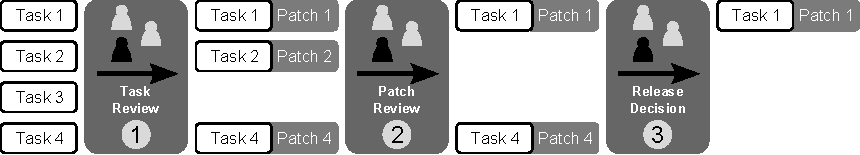
\includegraphics[width=\textwidth]{./figures/generalView}
  \caption{Main workflow followed by a task and the main points where decisions are made.}
  \label{fig:generalView}
\end{figure}

We have studied nine OSS projects where the participation is open to anyone willing to contribute, namely: Android\footnote{http://www.android.com}, GNOME\footnote{https://www.gnome.org}, 
Apache (web server) \footnote{https://www.apache.org}, Mozilla\footnote{https://www.mozilla.org}, Python\footnote{https://www.python.org}, Moodle\footnote{https://moodle.org}, EMF\footnote{https://www.eclipse.org/emf}, MoDisco\footnote{https://www.eclipse.org/modisco}. Table \ref{tab:comparative} shows a summary of the data we gathered. Next we describe the results in more detail.

\begin{table*}[t]
  \renewcommand{\arraystretch}{1.1}
  \centering
  \resizebox{\textwidth}{!}{%
    \begin{tabular}{|c|c|c|c|c|c|c|c|c|l|}\hline
    	\textbf{Project} & 
	\textbf{Organization} & 
	\textbf{Coordination} & 
	\textbf{Tracking system} & 
%	\textbf{Participation} & 
	\textbf{Task Review} & 
	\textbf{Patch Review} & 
	\textbf{Release Decision} & 
	%\textbf{Promotion} & 
	\textbf{Rules Def. / App.} &
	\begin{tabular}{c} \textbf{Roles} \end{tabular}\\ 
    \hline
 	Android &
	Hierarchy &
	Forum & 
	\begin{tabular}{c} Git \\ Gerrit \end{tabular} & 
%	Anyone & 
	\begin{tabular}{c} Yes \\ (Approver) \end{tabular} & 
	\begin{tabular}{c} Yes \\ (Verifier) \end{tabular} & 
	\begin{tabular}{c} Yes \\ (Project Lead) \end{tabular} & 
	%Selection & 
	\begin{tabular}{c} Documentation / \\ Track system\end{tabular} & 
	\begin{tabular}{l} Contributor \\ Developer \\ Verifier \\ Approver \\ Project Lead \end{tabular} \\
    \hline
        GNOME &
	Hierarchy & 
	\begin{tabular}{c} IRC \\ mailing-list \end{tabular} &
	Bugzilla &
%	Anyone &
	Yes &
	\begin{tabular}{c} Yes \\ (Bug Squad) \end{tabular} & 
	Yes &
	%Selection & 
	\begin{tabular}{c} Documentation / \\  Track System \end{tabular} & 
	\begin{tabular}{l} Contributor \\ Mentor \end{tabular} \\
%    \hline
%    	Joomla &
%	Hierarchy &
%	Forum &
%	\begin{tabular}{c} GitHub \\ Track \end{tabular} &
%	Anyone &
%	Yes &
%	\begin{tabular}{c} Yes \\ (Bug Squad) \end{tabular} & 
%	release &
%	%Selection &
%	\begin{tabular}{c} Implicit \\ (Documentation) / \\ Track System \end{tabular} & 
%	\begin{tabular}{l} Squads \end{tabular} \\
    \hline
	\begin{tabular}{c} Apache \\ Web \\ Server \end{tabular} &
	Meritocracy &
	Mailing-list &
	Bugzilla &
%	Anyone &
	\begin{tabular}{c} Yes \\ (Voting) \end{tabular} &
	\begin{tabular}{c} Yes \\ (Voting) \end{tabular} &
	\begin{tabular}{c} Yes \\ (Voting) \end{tabular} &
	% Selection &
	\begin{tabular}{c} Documentation / \\ Mailing-list \end{tabular} & 
	\begin{tabular}{l} User \\ Developer \\ Committer \\ PMC Member \\ PMC Chair \end{tabular} \\
%    \hline
%    	Linux   &
%	Hierarchy &
%	Mailing-list &
%	Git, Quilt & 
%	Anyone &
%	N/A &
%	N/A &
%	N/A &
%	%Selection &
%	\begin{tabular}{c} Implicit \\ Mailing-list \end{tabular} & 
%	\begin{tabular}{l} Any \end{tabular} \\
    \hline
    	Mozilla &
	Hierarchy & 
	\begin{tabular}{c} Forum \\ Mailing-list \\ IRC \end{tabular} &
	Bugzilla & 
%	Anyone &
	\begin{tabular}{c} Yes \\ (Module \\ Owner) \end{tabular} & 
	\begin{tabular}{c} Yes \\ (Module \\ Owner \& \\ Super-reviewers) \end{tabular} &
	\begin{tabular}{c} Yes \\ (Designated \\ Group) \end{tabular} &
	%Selection &
	\begin{tabular}{c} Documentation  / \\  Track System \& \\ Mailing-list \end{tabular} & 
	\begin{tabular}{l} User \\ Committer \\ Module Owner \\ Super-reviewer \end{tabular} \\
    \hline
    	Python &
	Hierarchy &
	\begin{tabular}{c} Mailing-list \\ IRC \\ Blogs \end{tabular} &
	\begin{tabular}{c} Mercurial \\ Roundup \end{tabular} &
%	Anyone &
	No &
	Yes (Reviewer) &
	\begin{tabular}{c} Yes \\ (Core Developer) \end{tabular} &
	%Selection & 
	\begin{tabular}{c} Documentation  / \\  Track System \end{tabular} & 
	\begin{tabular}{l} Contributor \\ Reviewer \\ Core Developer \end{tabular} \\
    \hline
    	Moodle &
	Hierarchy &
	Forum & 
	Moodle tracker &
%	Anyone & 
	\begin{tabular}{c} Yes \\ (Component \\ leads) \end{tabular} & 
	\begin{tabular}{c} Yes \\ (Developers) \end{tabular} &
	\begin{tabular}{c} Yes \\ (Component \\ Leads) \end{tabular} &
	%Selection & 
	\begin{tabular}{c} Documentation  / \\  Track System \end{tabular} & 
	\begin{tabular}{l} Users \\ Developers \\ Component Leads \\ Integrators \\ Testers \\ Manteiners \end{tabular} \\
    \hline
    	EMF &
	Hierarchy &
	Forum &
	Bugzilla & 
%	Anyone &
	\begin{tabular}{c} Yes \\ (Committer) \end{tabular} & 
	\begin{tabular}{c} Yes \\ (Committer) \end{tabular} & 
	\begin{tabular}{c} Yes \\ (Project Leader) \end{tabular} & 
	%Selection &
	\begin{tabular}{c} Documentation  / \\  Track System \end{tabular} & 
	\begin{tabular}{l} User \\ Contributor \\ Committer \\ Project Leader \end{tabular} \\
    \hline
    	MoDisco &
	Hierarchy &
	Forum &
	Bugzilla &
%	Anyone & 
	\begin{tabular}{c} Yes \\ (Committer) \end{tabular} &
	\begin{tabular}{c} Yes \\ (Committer) \end{tabular} &
	\begin{tabular}{c} Yes \\ (Committers) \end{tabular} &
	%Selection &
	\begin{tabular}{c} Documentation  / \\  Track System \end{tabular} & 
	\begin{tabular}{l} User \\ Contributor \\ Committer \\ Project Leader \end{tabular} \\
    \hline
  \end{tabular}}
  \caption{Comparison of how OSS systems are governed.}
  \label{tab:comparative}
\vspace{-0.25cm}
\end{table*}

\vspace{0.15em}
\noindent \textbf{Organization}. The organization followed by a project summarizes its main development philosophy. The great majority of analyzed projects follow a hierarchical scheme, thus meaning that there exist several hierarchical levels in the groups of users collaborating in the development (e.g., leaders, contributors, users, etc.). Thus, there are several roles (see the corresponding feature below) which a user can belong to. A good example is the Android project, where each role has assigned a particular function in the process (e.g., \textit{approvers} approve tasks, \textit{verifiers} review patches, etc.) supporting the project leader. On the other hand, Apache differs from the others by using a meritocracy organization where users can gain merits as they contribute to the project. 

\vspace{0.15em}
\noindent \textbf{Coordination}. This feature includes the main tools used to help users to collaborate during the development process. As can be seen, mailing-list and forums are the main tools used. Note that even though these tools are useful to keep in touch with the rest of developers, they are normally used to apply some governance rules as well, which goes beyond the original purpose of those tools. This is the case of Apache, which uses a mailing-list to vote which issues/bugs should be implemented/fixed next.

\vspace{0.15em}
\noindent \textbf{Tracking system}. The managament of tasks is performed by tracking systems, Bugzilla being the most popular one. Interestingly enough, tracking systems are also used as a forum-like tool to discuss possibles tasks which are not mature enough to be considered as real issues. For instance, in the GNOME project, some tasks\footnote{http://felipec.wordpress.com/2011/09/23/no-gnome-doesnt-want-user-feedback-how-i-argued-in-favor-of-voting-in-bugzilla-and-got-banned-as-a-result} in Bugzilla are used to openly discuss possible changes in the development strategy.

%  \item \textbf{Participation}. In general, in OSS systems, anyone is able to take part in the development, i.e. it is not necessary to be an official developer to inform new issues or bugs. 

\vspace{0.15em}
\noindent \textbf{Task review}. Once a task (i.e., issue/bug) is notified, it can be reviewed to be accepted or rejected. Except for Python, where all the task are accepted and only reviewed if they include the corresponding patch, the rest of the projects have a decision process to accept or reject the task proposal. In general, the decision process is made by either the leader (e.g., component leaders in Moodle) or by unanimous agreement if there are several leaders (e.g., in big Eclipse-based projects such as EMF).

\vspace{0.15em}
\noindent \textbf{Patch review}. Tasks have attached the corresponding patch implementing the improvement (if it is an issue) or the fix (if it is a bug). Before incorporating the patch into the product, it is possible to perform a revision and test to check the quality of the patch. All the analyzed projects include a review process which analyzes the patch and eventually decides its acceptance or rejection.

\vspace{0.15em}
\noindent \textbf{Release Decision}. As the tasks and the corresponding patches are accepted, new software product releases have to be published. In the vast majority of analyzed projects, the decision of selecting when to perform the release and which tasks should be incorporated normally is taken by the product/component leader or by unanimous agreement when there are several leaders. The only exception is the decision process for Apache, where a ballot takes place.

\vspace{0.15em}
\noindent \textbf{Governance rule definition and application}. This feature shows how governance rules are defined and applied. In general, none of the projects explictly defines these rules, and the result of their application is scattered througout the management systems (i.e., track systems or mailing-lists).

%  \item \textbf{Promotion}. This feature describes how people can gain specific roles in the community. All the projects analyzed applies a selection process where a leader chooses who should change the role. Only in the Apache community, the selection process is performed by voting.

\vspace{0.15em}
\noindent \textbf{Roles}. The users collaborating in the development are classified according to a set of roles. All the analyzed projects include both the role of developer (also known as contributor or commiter), who can commit changes into the source code repository of the project and the corresponding role for leaders (also known as owners or chairs).

In summary, most projects are hierarchical where a group of contributors are driven by a leader (or a set of leaders) who normally decides which tasks should be completed first. Patches are normally reviewed and tested by contributors while the product release is decided by a leader group as well. Thus, the resulting governance rules are mainly controlled by the group of leaders, who can decide how the software product should evolve. When there is a group of leaders, the decision is normally made by unanimous agreement and normally using tools such as email, mailing-lists or forums. 

The development of Apache web server is the main exception. The project is governed by a vote-based strategy where all the contributors can decide which tasks should be accepted and which ones should be included into the final release. It is important to note that although anyone can vote, only the votes from contributors are binding, the rest are helpful to see the general opinion of the community. The project also establishes how the voting should be performed. Thus, if the task involves changes in the source code, the voting should unanimously agree to make the change and at least three votes must be casted. Otherwise, if the change does not involve code, a majority of positives votes (and at least three) are required. Moreover, any negative vote must include the corresponding rationale, which can therefore help to solve the disagreement.

Interestingly enough, in all the analyzed projects it was not trivial for us to discover the governance rules being applied since the available information was scarce and normally scattered among the documentation of the project. In fact, some projects such as GNOME recommend to be patient since it can take a long time to become a contributor. Potential contributors are therefore required to observe existing mailing lists, conversations on IRC, etc. to discover the way of working in the project. 

Moreover, the result of the application of these rules is directly updated in the tracking systems, where normally there is no tracking information that helps to clarify later on why that decision was taken nor the possible discussion threads (maybe taken place outside the tracking systems, e.g., by chat or email as it is the case for smaller projects such as MoDisco) among the leaders that lead to that decision. 

Clearly, making explicit the governance rules followed in a project could help the developer community to understand and apply those rules as part of their daily development activities. Next sections describe our proposal to tackle this problem.



\section{Overview of Our Approach}
\label{sec:approach}
Our proposal consists in two main components. First, to make the governance rules explicit, we propose to use a Domain Specific Language (DSL) including concrete constructs to define which decision rules must be followed to act on a set of tasks/patches. Secondly, we propose to enable the ``execution'' of the DSL specifications so that, beyond improving the understanding of the project internal organization, they can also be used to support and guide the collaboration among the project participants.

We believe our DSL would be useful in all the decision points identified before. Figure \ref{fig:process} illustrates how the application of our DSL would change the group dynamics in a particular decision point. As can be seen, given a set of tasks to be discussed in a decision point (i.e., either to accept them, accept a patch for them or include them in a release), users can vote for/against them (step 1), a decision engine analyzes the votes according to the governances rules defined (e.g., total agreement, simple majority, etc.) (step 2). As a result, the status of the tasks is changed based on the decisions taken by the engine (step 3). 

\begin{figure}[t]  
  \centering
  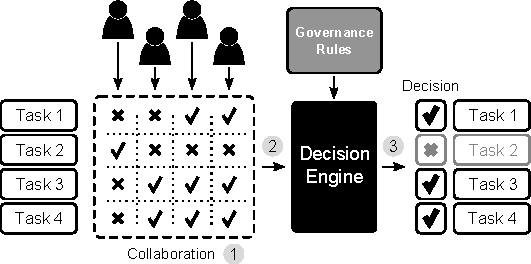
\includegraphics[width=0.6\textwidth]{./figures/processB}
  \caption{Decision process proposed.}
  \label{fig:process}
\end{figure}

In what follows we define the DSL and the infrastructure required to enable its use in practice in more detail.




\subsection{A DSL to Define Governance Rules}
\label{sec:dsl}
A DSL is defined by three main elements \cite{bib:kleppe}: abstract syntax, concrete syntax and semantics. The abstract syntax defines the main concepts and their relationships, and also include well-formedness rules constraining how the concepts and relationships have to be used. The concrete syntax defines the language notation (textual, graphical or hybrid) and a translational approach is normally used to provide semantics.

Our DSL has been defined in the context of Model-Driven Engineering, thus we used metamodelling techniques \cite{bib:Brambilla} to define the abstract syntax. A metamodel formally describes the structure of the models which are used to represent an aspect of a system at some abstraction level. In our case, we have defined a metamodel to represent the concepts and relationships needed to define governance rules. A model is an instance of a metamodel, and the \emph{conforms to} term is normally used to express this \emph{instance of} relationship between models and metamodels. Thus, models of our language conform to the language abstract syntax metamodel and represent specific instances of governance rules. As concrete syntax, we have opted for a textual language following a typical block-based structure. Thus, each instance of a metaclass is represented by its keyword and a block which contains the name and value of its attributes. Containment references are represented as nested blocks while non-containment references use an identifier to refer the referred element. In the following we will show some examples to illustrate the syntax.

\begin{figure*}[t]
\centering
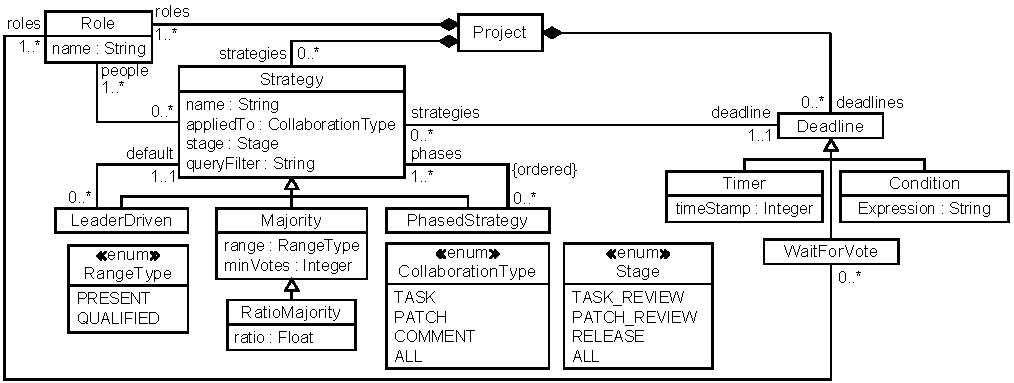
\includegraphics[width=\textwidth]{./figures/decisionStrategy}
\caption{Abstract syntax metamodel of our DSL to represent governance rules (expressed as a UML class diagram).}
\label{fig:decisionStrategy}
\end{figure*}

The abstract syntax metamodel of the language is shown in Figure \ref{fig:decisionStrategy}. The concepts represented in the metamodel covered all the governance aspects identified in our study of OSS projets (Section \ref{sec:motivation}). In particular, a development project (\texttt{Project} metaclass) includes a group of roles of users (\texttt{roles} reference), strategies (\texttt{strategies} reference) and deadlines (\texttt{deadlines} reference). A role has an identifier (\texttt{id} attribute in \texttt{Role} metaclass) and represents a group of people in the development community who can vote. Decision strategies are applied to a particular type of collaborations (\texttt{appliedTo} attribute) according to their nature in the track system (i.e., task, patch or comment) and at a concrete moment (\texttt{stage} attribute) of the process (i.e., task review, patch review, and release). The scope of the strategy can also be defined (\texttt{queryFilter} attribute) (e.g., only those ones which are tagged as high priority). We have defined several decision strategies (included in the hierarchy with root \texttt{Strategy}), which cover the following:

\vspace{0.15em}
\noindent \textbf{Majority Strategy}. This decision strategy (\texttt{Majority} metaclass) accounts for the number of votes received by a collaboration element. Thus, only those elements which have received a support greater than 50\% will be selected. The way of counting votes may differ depending on who is available in the moment of the votation. Since different terminology is used to refer the several types of majority (e.g., \emph{plurality} or \emph{relative majority} used in North America is called \emph{simple majority} in Europe), we will use the neutral term \emph{majority range} to determine exactly how the votes should be counted. Thus, if the range is \texttt{present}, the majority is based on those participants that are present in the moment of voting. Otherwise, a \texttt{qualified} range is based on those participants qualified to vote (presently available or not). A majority strategy can also require a minimum number of votes to be triggered (\texttt{minVotes} attribute). 
    
    As an example, a majority strategy to be applied only to tasks, voted by the committers if they are presently available,  with no need of minimum votes and with a deadline of seven days from the task creation date would be specified as shown in Figure \ref{fig:strategies}a.

\begin{figure*}[t]
\centering
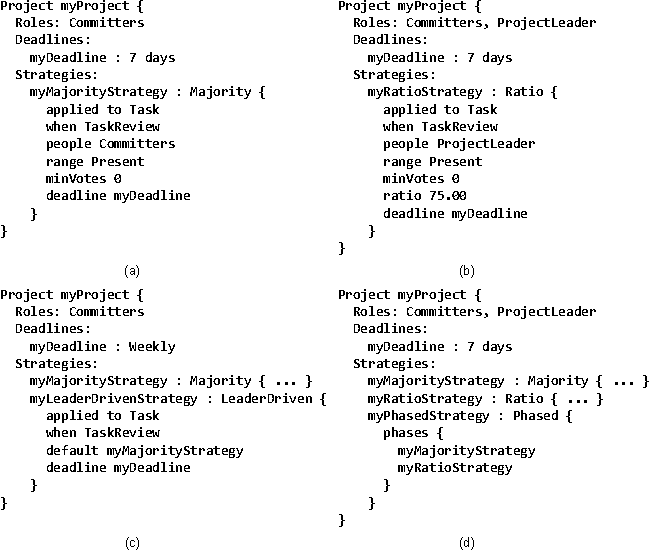
\includegraphics[width=0.8\textwidth]{./figures/strategies}
\caption{Examples of decision strategies: (a) Majority strategy, (b) Majority strategy using ratio (c) Leader-Driven Strategy, (d) Phased Strategy.}
\label{fig:strategies}
\end{figure*}

%{\scriptsize
%\begin{verbatim}
%Project myProject {
%  Roles: Committers
%  Deadlines:
%    myDeadline : 7 days
%  Strategies:
%    myMajorityStrategy : Majority {
%      applied to Task
%      when TaskReview
%      people Committers
%      range Present
%      minVotes 0
%      deadline myDeadline
%    }
%}
%\end{verbatim}
%}

A different percentage for the majority can also be set. In this case the strategy will be called ratio majority (\texttt{RatioMajority} metaclass) and the ratio value must be specified. For instance, this type of strategy would allow implementing well-known majorities such as three-fifths or two-thirds, which may be required for changes on fundamental laws. As example of ratio majority, the definition shown in Figure \ref{fig:strategies}b modifies the strategy presented before to be ratio-based with a ratio of acceptance of 75\% and to be voted only by the project leaders.

%{\scriptsize
%\begin{verbatim}
%Project myProject {
%  Roles: Committers, ProjectLeader
%  Deadlines:
%    myDeadline : 7 days
%  Strategies:
%    myRatioStrategy : Ratio {
%      applied to Task
%      when TaskReview
%      people ProjectLeader
%      range Present
%      minVotes 0
%      ratio 75.00
%      deadline myDeadline
%    }
%}
%\end{verbatim}
%}

\vspace{0.15em}
\noindent \textbf{Leader-Driven Strategy}. When the decision of accepting a collaboration element relies on a user playing the role of leader (e.g., component or project leader), a leader-driven strategy (\texttt{LeaderDriven} metaclass) is followed. Thus, this decision strategy relies on the leader of a collaboration element to decide its acceptance. Next section describes how the leader is represented. The leader must also define a default strategy (\texttt{default} reference) where to delegate the decision in case the leader is not available (i.e. the leader doesn't vote before the deadline)
  
Figure \ref{fig:strategies}c shows an example of leader-driven strategy to be applied only to tasks, with a majority default strategy to be applied when the leader does not make the decision and with a deadline of seven days from the task creation date would be (note that the \texttt{myMajorityStrategy} strategy defined before is reused as default behavior).

%{\scriptsize
%\begin{verbatim}
%Project myProject {
%  Roles: Committers
%  Deadlines:
%    myDeadline : Weekly
%  Strategies:
%    myMajorityStrategy : Majority { ... }
%    myLeaderDrivenStrategy : LeaderDriven {
%      applied to Task
%      when TaskReview
%      default myMajorityStrategy
%      deadline myDeadline
%    }
%}
%\end{verbatim}
%}

\vspace{0.15em}
\noindent  \textbf{Phased Strategy}. This is a composite strategy which allows applying several strategies in a chained way. The strategies are defined and applied in an ordered way (\texttt{phases} reference). Thus, a set of collaboration elements are selected according to the first strategy, the selected ones are then voted again and filtered according to the second strategy, and so on. 

    An example of phased strategy composed of two phases where the first one applies a majority among the committers and with a deadline of seven days from the task creation date, and the second phase, which has a deadline of seven days after the first phase has been done, applies a leader-driven strategy among the project leaders would be (note that \texttt{mymajorityStrategy} and \texttt{myRatioStrategy} are reused) is shown in Figure \ref{fig:strategies}d.

%{\scriptsize
%\begin{verbatim}
%Project myProject {
%  Roles: Committers, ProjectLeader
%  Deadlines:
%    myDeadline : 7 days
%  Strategies:
%    myMajorityStrategy : Majority { ... }
%    myRatioStrategy : Ratio { ... }
%    myPhasedStrategy : Phased {
%      phases {
%        myMajorityStrategy
%        myRatioStrategy 
%      }
%    }
%}
%\end{verbatim}
%}



Regarding the deadlines that trigger a decision strategy, we have currently defined three covering deadlines based on: (1) time (\texttt{Timer} metaclass), (2) a condition to be fulfilled in the collaboration (\texttt{Condition} metaclass) (e.g., the change of a tag in the collaboration model) and (3) a set of users have voted (\texttt{WaitUserVote} metaclass).
 


\subsection{Applying Governance Rules} 
\label{sec:collaboration}
To be able to use the governance rules to manage the project we need to: (1) provide support for the recording of the information generated by all the participants interactions (e.g., proposals, votes, etc.), and (2) implement a decision engine that can use this information and apply the governance rules to make the corresponding decisions. 

To record the participant's interactions we use the schema shown in Figure \ref{fig:collaboration}. A particular collaboration (\texttt{Collaboration} metaclass) is represented by an identifier (\texttt{id} attribute) and a rationale explaining the collaboration (\texttt{rationale} attribute). There are three types of collaboration elements (\texttt{type} attribute in \texttt{Collaboration} metaclass): tasks, which represent a request for an issue or a bug; patches, which represent the solution for a task; and comments, which represent comments that users can make to other collaborations. A collaboration element can also have some metadata information (\texttt{metadata} reference) and has a proposing user (\texttt{isProposed} reference) and a leader (\texttt{leader} reference). During the collaboration, a user (\texttt{User} metaclass) is identified by an identifier (\texttt{id} attribute) and belongs to a one or more roles (\texttt{roles} reference).  Note also that both collaboration elements and users are linked to the tracking system (see \texttt{Tracking System} component) to retrieve the information of tasks/patches/comments and users, respectively. The metamodel also allows representing votes (\texttt{Vote} metaclass) from the users, which can agree/disagree with a collaboration (\texttt{agreement} attribute). A vote has a timestamp (\texttt{timeStamp} attribute) and a rationale (\texttt{rationale} attribute) explaining the reason for the positive/negative vote. 


\begin{figure*}[!t] 
  \centering
  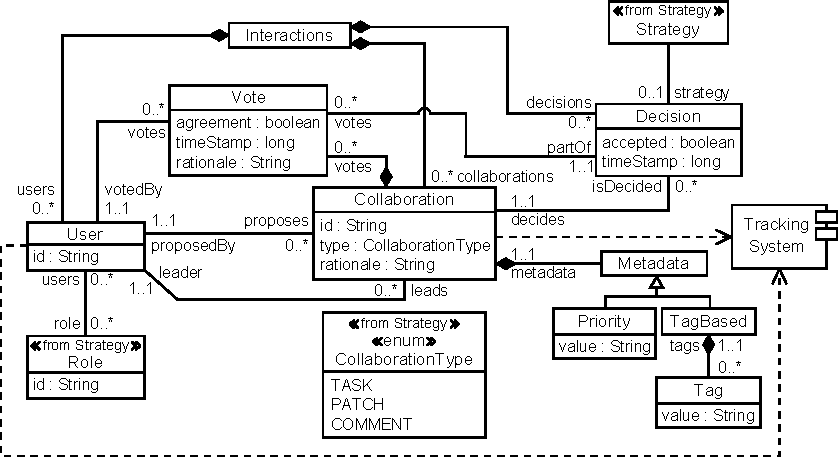
\includegraphics[width=0.8\textwidth]{./figures/collaboration}
  \caption{Metamodel to represent collaborations.}
  \label{fig:collaboration}
\end{figure*}

When the deadline for a governance rule passes, the decision engine receives the collaboration model as input and follows the rule instructions to process the data and take a decision. The decision updates the collaboration information to create the new decisions (\texttt{Decision} metaclass) and trace them back to the affected collaboration elements (\texttt{isDecided} reference). A decision can accept/reject a collaboration element (\texttt{accepted} attribute), includes a timestamp of the moment when the decision was made (\texttt{timeStamp} attribute) and refers to the strategy applied (\texttt{strategy} reference). A collaboration element has usually only decision element assigned except when a phased strategy is used, in this case the decisions for each phase and the final decision are also stored in the model. The decision engine is provided as part of our prototype tool implementation (see Section \ref{sec:implementation}).



\section{Case Study: Apache}
\label{sec:example}
We have used our approach to model the decision process applied in the Apache project (the choice of Apache was motivated by the fact that it has a more complex governance process than other analyzed projects). 

We first represent the governance rules used to select tasks to accomplish. As described before, there are two types of voting procedures depending on whether the task to accomplish involves source code changes or not. The DSL defining the Apache governance rules is listed in Figure \ref{fig:rulesApache}.

\begin{figure}[t]
  \centering
  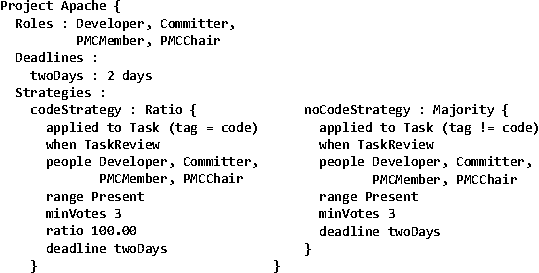
\includegraphics[width=0.65\textwidth]{./figures/apache}
  \caption{Apache governance rules.}
  \label{fig:rulesApache}
\end{figure}


%{\scriptsize
%\begin{verbatim}
%Project Apache {
%  Roles : Developer, Committer,
%          PMCMember, PMCChair
%  Deadlines :
%    twoDays : 2 days 
%  Strategies :
%    codeStrategy : Ratio { 
%      applied to Task (tag = code)
%      when TaskReview
%      people Developer, Committer, 
%             PMCMember, PMCChair
%      range Present
%      minVotes 3 
%      ratio 100.00 
%      deadline twoDays 
%    }, 
%    noCodeStrategy : Majority {
%      applied to Task (tag != code)
%      when TaskReview
%      people Developer, Committer, 
%             PMCMember, PMCChair
%      range Present
%      minVotes 3  
%      deadline twoDays
%    }
%}
%\end{verbatim}
%}

The example defines four roles and two strategies called \texttt{codeStrategy} and \texttt{noCodeStrategy}. The former is a ratio majority strategy which is applied to those tasks including the tag \texttt{code} (i.e., tasks involving changes in the code). All people belonging to the roles linked to the strategy (see tag \texttt{people}) and presently available (see tag \texttt{range}) can vote. It is required a ratio of agreement of 100\% (i.e., meaning that everybody has to agree) and at least three votes. Finally, the strategy defines a deadline of two days, although the precise length is not specified in the project documentation. On the other hand, \texttt{noCodeStrategy} is a majority strategy which is applied to those tasks not including the tag \texttt{code}. Like the previous strategy, it is required at least three votes to make a decision and the deadline is two days after the creation of the task. 

As an example of applying the previous rules, Figure \ref{fig:exampleCollaborationApache} shows a possible collaboration model representing how developers made the decision about two task proposals with identifier \texttt{task1} and \texttt{task2}. The former includes the tag \texttt{code} while the latter does not, thus allowing illustrating the application of both governance rules (i.e., \texttt{codeStrategy} rule for the first task and \texttt{noCodeStrategy} rule for the second one). For the sake of the clarity and conciseness, the \texttt{rationale} and \texttt{timeStamp} attributes have been removed in the Figure. As can be seen, after voting, although the first task has received more than three votes, it it is rejected because there is at least one vote negative. On the other hand, the second task is accepted because, although there is a negative vote, the majority of them agrees with the change. 

Note that instead of the current process (based on mail communications and manual counting of the votes) our approach (and related tool support) automatically takes the decisions based on the rules and the interactions taking place between the developers. Moreover, both the collaboration and decisions are stored in along with the element decided (i.e., the task status change), thus avoiding scattering information along the project management tools (i.e., the mailing-list in this case) and improving the transparency of the process.

\begin{figure}[t]
  \centering
  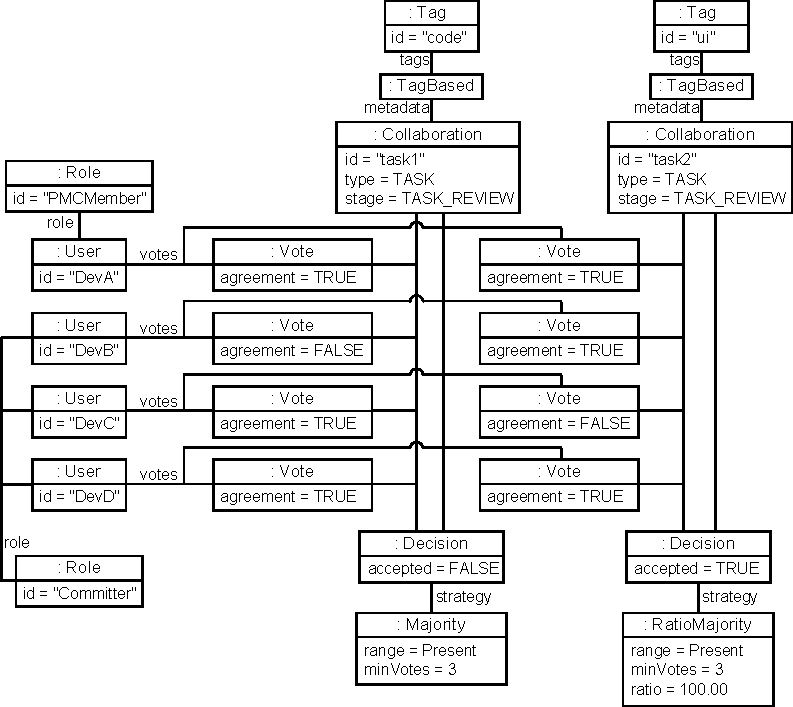
\includegraphics[width=0.65\textwidth]{./figures/exampleCollaborationApache}
  \caption{Example of collaboration in Apache.}
  \label{fig:exampleCollaborationApache}
\end{figure}

%In this section we present an example to illustrate the DSL and the collaboration that may arise. Imagine a development process where the main development tasks are selected according to a democratic process where the developers can participate. The decision process is divided into two phases. During the first phase, the developers team have two hours to vote for/against which existing development tasks should be accomplished, only those ones with a third of simple majority will be selected. In the second phase, those tasks selected in the previous phase are taken into consideration by a committee composed of three senior developers. The committee can must vote for/against the tasks so that only those ones with absolute majority will be selected, in any time the main leader of the team can select the tasks which are urgent, thus avoiding to be voted by yhe senior developers.

%{\footnotesize
%\begin{verbatim}
%Project example {
%  Roles: Developer, Boss, SuperBoss
%  Strategies:
%    myRatioExamples : Ratio {
%      applied to Proposal
%      people Developer
%      range Present
%      minVotes 0
%      ratio 0.66
%    }
%    myMajorityExample : Majority {
%      applied to Proposal
%      people Boss
%      range Present
%      minVotes 0
%    }
%    myPhasedStrategy : Phased {
%      applied to Proposal
%      phases myMajorityExample, 
%             myRatioStrategy
%    }
%}
%\end{verbatim}
%}


%Figure \ref{fig:exampleStrategy} shows the decision strategy model expressed by our DSL for the example. As can be seen, the main decision strategy is a phased strategy (see instance of \texttt{PhasedStrategy} metaclass) composed of two phases. The first phase is an instance of \texttt{RatioMajority} metaclass which considers all the developers as voters, its \texttt{type} attribute is set to \texttt{SIMPLE} to indicate that the majority is simple and its \texttt{ratio} attribute is set to \texttt{0.66} specifying the proportion to fulfill. The deadline for this phase is a \texttt{Timer} instance whose \texttt{mins} attribute is set to \texttt{120} (i.e., two hours). On the other hand, the second phase is an instance of \texttt{LeaderDriven} metaclass which assigns the role of leader to the main team developer (see \texttt{User} metaclass instance with \texttt{id} attribute set to \texttt{SuperBoss}) and its deadline is a \texttt{WaitUserVote} to indicate that the strategy has to wait for the vote of the leader. The default behavior for this strategy is referring to an instance of \texttt{Majority} metaclass with its \texttt{type} attribute set to \texttt{ABSOLUTE} to indicate that the majority is absolute and the users involved are the three senior developers (see \texttt{User} metaclass instances with \texttt{id} attributes set to \texttt{BossA}, \texttt{BossB} and \texttt{BossC}).

%\begin{figure}[t]
%  \centering
%  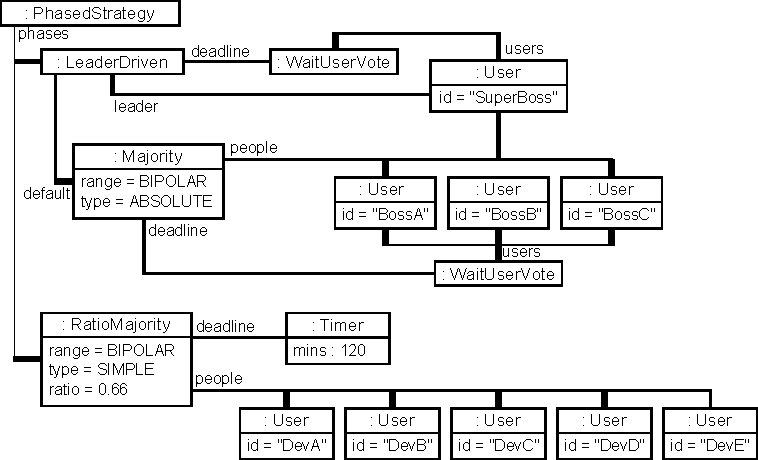
\includegraphics[width=\columnwidth]{./figures/exampleStrategy}
%  \caption{Example of decision strategy}
%  \label{fig:exampleStrategy}
%\end{figure}

%As an example of executing the decision strategy, Figure \ref{fig:exampleCollaboration} shows a possible scenario where team developers have to make a decision about a task proposal with identifier \texttt{task1}. As can be seen, the first phase involves the vote of the developers: users with identifiers \texttt{DevA}, \texttt{Devb} and \texttt{DevC} vote possitively, user with id \texttt{DevD} votes negatively and user with identifier \texttt{DevE} does not vote. The result of the first phase is the aceptance of the proposal to be accomplished so it is then triggered the second phase of the strategy. In the second phase, the leader votes for the proposal so there is on need to make a votation with the senior developers. Thus, the final decision is to accept the proposal.

%\begin{figure}[t]
%  \centering
%  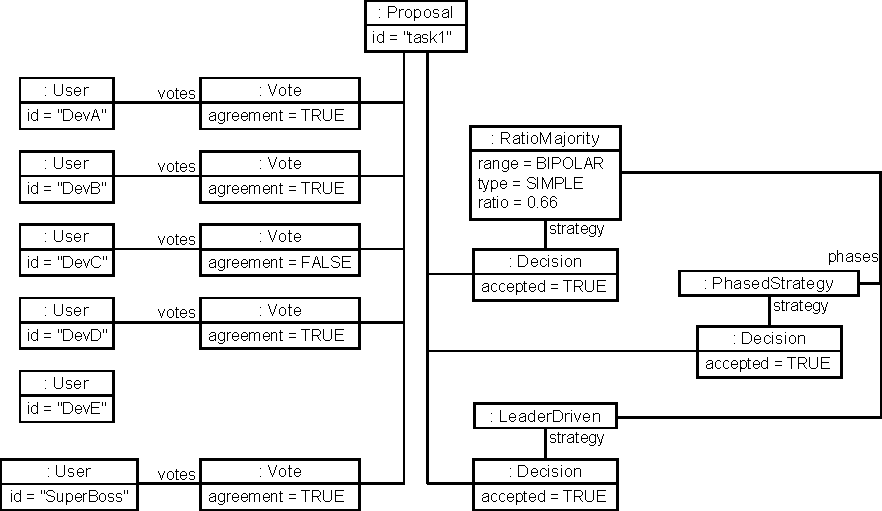
\includegraphics[width=\columnwidth]{./figures/exampleCollaboration}
%  \caption{Example of collaboration}
%  \label{fig:exampleCollaboration}
%\end{figure}





\section{Implementation}  
\label{sec:implementation}
\begin{figure*}[t] 
  \centering
  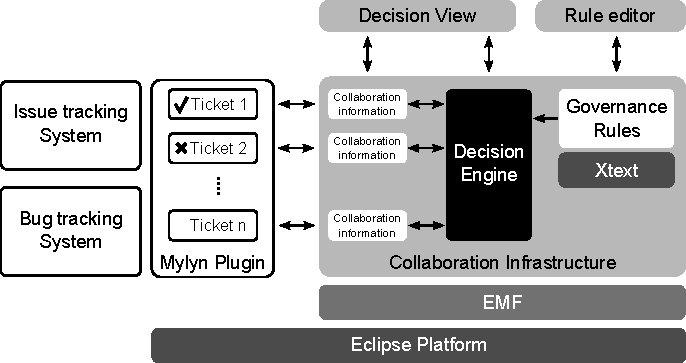
\includegraphics[width=0.65\textwidth]{./figures/architecture}
  \caption{Architecture of the developed tool.}
  \label{fig:architecture}
\end{figure*}


Our approach has been implemented as an Eclipse plug-in \footnote{The prototype can be downloaded from https://code.google.com/a/ eclipselabs.org/p/governance-rules-mylyn/} providing a collaborative infrastructure allowing developers and project managers to define and apply governance rules. 

Figure \ref{fig:architecture} summarizes the architecture of our prototype tool. We rely on Mylyn\footnote{http://www.eclipse.org/mylyn} for accessing and updating the tasks of the development project we are collaborating on. Mylyn incoporates several connectors covering a great variety of tracking systems\footnote{The complete list of supported tools can be found at http://wiki.eclipse.org/index.php/Mylyn\_Extensions}. The collaboration models storing all the information about the ongoing discussions, votes, etc. are implemented on top the EMF \footnote{http://www.eclipse.org/emf} Eclipse component. 

Our DSL to define governance rules has been developed in Xtext\footnote{http://www.eclipse.org/Xtext}, a tool to create textual DSLs in Eclipse. In Xtext, DSLs are described by an annotated grammar from which the required tooling is generated (e.g., specific editor, syntax highlighting, auto-completion, content assistance, etc.). We defined the grammar for our DSL and generated the corresponding DSL tooling. The plugin therefore provides a specific editor to define governance rules (see \emph{Rule editor}). 

Once the rules are defined, the collaboration information is collected in a dedicated view (see \emph{Decision View}) and, via Mylyn, linked to the project tasks as metadata. The rules plus this information are then interpreted by an engine developed in Java (see \emph{Decision Engine}) that updates the tasks status according to the governance rules defined.

Figure \ref{fig:snapshot} shows a snapshot of the platform including both the \emph{Decision view} (on the left bottom part) and the \emph{Rules editor} (on the right top part) for the Apache example presented before. Five tasks from the Apache repository (project \texttt{apache-httpd-2}) have been selected for the sake of conciseness. As can be seen, these tasks are shown in the \emph{Task List} view provided by Mylyn and in the \emph{Decision view} provided by our tool, which allows users to vote for/against these tasks. The view also includes buttons to configure the strategy (opening the \emph{Rule editor} shown in the Figure), to apply it, to login and to refresh the view. As an example, the rules have been triggered using sample votes, thus resulting in the acceptance of the first two tasks and rejection of the rest. 

\begin{figure*}[t] 
  \centering
  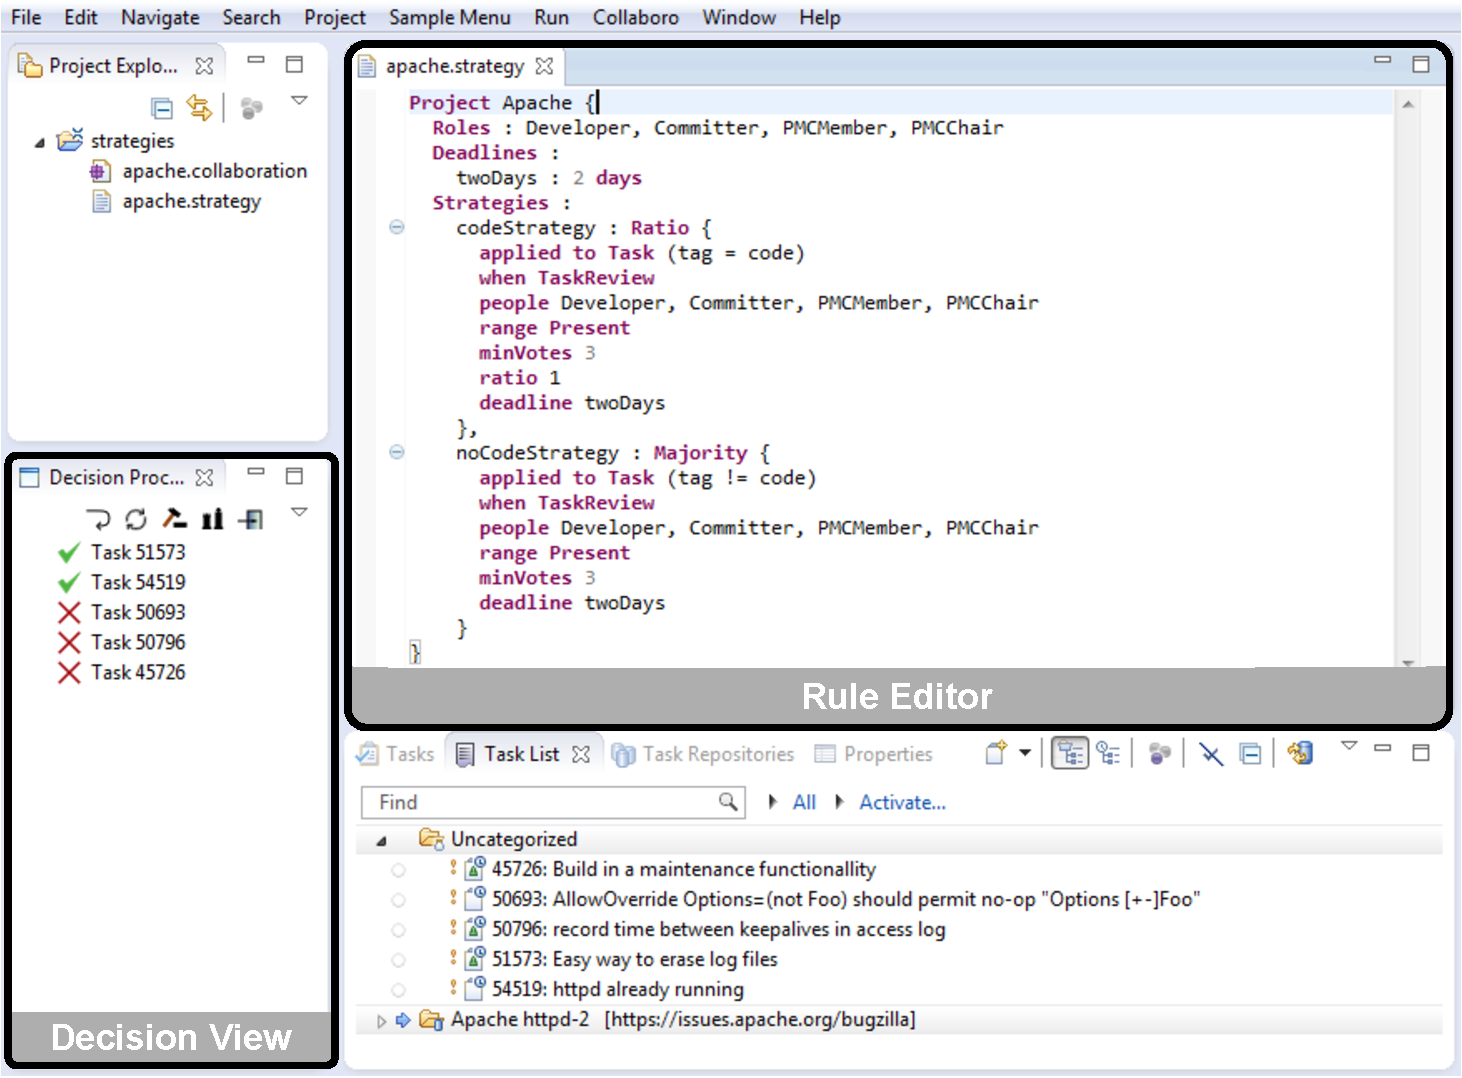
\includegraphics[width=0.85\textwidth]{./figures/snapshot}
  \caption{Snapshot of the developed tool.}
  \label{fig:snapshot}
\end{figure*}



\section{Related Work} 
\label{sec:relatedWork}
The study of how people coordinate to develop a software system has been a research topic for a long time~\cite{Herbsleb1999,Kraut1995,Parnas1972,Crowston2005,Markus2007}, including the broader topic of IT governance \cite{Chulani2008,Ramasubbu2008,sg,Webb2006}. In the field of software governance in OSS, several works have tried to classify how these projects are managed \cite{Laat2007,Markus2007,DeNoni2013}. However, to the best of our knowledge, little attention has been paid to the precise definition and support for the governance rules in specific projects.

Some works report on concrete case studies. For instance, \cite{Aranda2009} reports on the coordination activities performed to solve bugs (e.g., how bugs are detected and closed, means used to coordinate the work, etc.). In \cite{Guzzi2013} authors present how developers use mailing list during the development of FLOSS systems (e.g., which are the main topics discussed or the level or participation of the different user roles). In \cite{osswatch} some indications are provided to describe governance models in natural language.

Other approaches focus on leveraging collaboration information obtained by mining software repositories to infer coordination relationships and structures.  The work presented in \cite{Bird2008} describes an approach to discover potential social structures from the threads created in the mailing list of the project. In \cite{Heller2011} visualization techniques are applied to easily discover communication patterns from Github repository metadata (e.g., the effect of geographic distance among developers, influence among cities, etc.). The tool called CrowdWeaver is present in \cite{Kittur2012}, which allows coping with the complexity of managing crowdsourced projects. These tools could be adapted to facilitate the discovery of governance rules using our approach.

Concrete methodologies for collaboration strategies have also been proposed. For instance, \cite{Duque2012} and \cite{Luther2013} present approaches to support collaborative processes in groupware systems and online creative projects, respectively. However, they do not provide mechanisms to define and apply the governance rules to apply in each project.

Collaboration has also been the focus on two other DSLs. The approach presented in \cite{Gallardo2012} describes a DSL to represent collaboration workflows that can appea in modeling tools (e.g., the steps needed to create a class diagram when several users are collaborating). In our previous work \cite{bib:collaboro} we presented a DSL-based tool to collaborativelly develop DSLs, thus allowing representing the collaborations arisen in the process. Again, they do not provide any support for the governance of such collaborations.



\section{Conclusion} 
\label{sec:conclusion}
In this paper we have presented an approach that opens the possibility to explicitly define and automatically aply the rules that govern a software development project. Our approach includes a new DSL for specifying the rules, a collaboration infrastructure to record the interactions (and to be able to trace them back) and a decision engine to automatically update the tasks status based on that. A prototype tool implemented as an Eclipse plug-in and relying on the Mylyn component for the connection with the most popular tracking systems has been developed. Note that although our approach supports both the definition and application of governance rules, they can be used independently and project leaders can therefore decide using only the former, which would improve the transparency and sustainability of governance model.

%As a direct application of our approach, we plan to use it to improve our DSL itself. By using a tracking system, users can request language improvements (e.g., including new constructs, modifying keywords, etc.) that are then voted and decided according to governance rules which have been defined explicitly\footnote{The project is located at http://}. 

As further work, we would like to provide support for evolution in governance rules as they depend on social interactions it is common to find temporal exception, ambiguities and changes over time.
%extend our rule definition language to be able to specify as well the rules governing the team organization (e.g., how the project participants can be promoted between the different roles). 
Adding privacy concerns is also under evaluation (some projects may require anonimity in the votation phase, or keep private some discussions to all people with less privileges). Finally, we would like to mine existing software repositories to infer and study the governance rules they are using. It would be interesting to see if the extracted rules correspond to the perception of (external) participants (e.g., whether they have evolved through time or whether their application is full of exceptions) and how they correlate with other metrics of the projects.


\bibliographystyle{splncs}
\bibliography{caise2014-governance}

\end{document}


